\documentclass{article}
\usepackage{polski}
\usepackage{blindtext}
\usepackage{amsmath}
\usepackage{mathtools}
\usepackage{graphicx} 
\usepackage{wrapfig}
\usepackage{amssymb}
\usepackage{multirow}
\usepackage[usenames,dvipsnames,svgnames,table]{xcolor}
\usepackage{float}
\usepackage[caption = false]{subfig}
\usepackage{caption}
\newcommand\tab[1][1cm]{\hspace*{#1}}
\usepackage[a4paper, left=2cm, right=2cm, top=2cm, bottom=2cm, headsep=1.2cm]{geometry}

\usepackage{titling}
\newcommand{\subtitle}[1]{%
  \posttitle{%
    \par\end{center}
    \begin{center}\large#1\end{center}
    \vskip0.5em}%
}


\begin{document}
\title{Aproksymacja sygnału okresowego przy użyciu FFT}
\author{Wiktoria Zaczyk}
\date{20.05.2020}

\maketitle	

\section{Wstęp teoretyczny}
\textbf{Dyskretna transformata Fouriera (DFT)}
\newline
transformata Fouriera wyznaczona dla sygnału próbkowanego, a więc dyskretnego. Obliczanie sum ma złożoność obliczeniową $ O(N^2)$ dla liczb zespolonych $a_0,a_1,...,a_n_-_1$ i $k=0,1,..,N-1$ określonych wzorem:
\begin{equation}
\begin{array}{c}
A_k = \displaystyle \sum _{n=0}^{N-1}(a_ne^-^\frac{2\pi i}{N}^n^k) 
\end{array}
\end{equation}
\newline
\textbf{Szybka transformata Fouriera (FFT)}
\newline
Szybką transformacją Fouriera nazywamy algorytm wyznaczania dyskretnej transformaty Fouriera oraz transformaty do niej odwrotnej. Pozwala on zmniejszyć liczbę wykonywanych operacji do $O(N log_2N)$ 
\newline\newline
\textbf{Algorytm radix-2}
\newline
Jest to najprostszy algorytm FFT. W algorytmie tym zakładamy, że całkowita liczba węzłów to potęga 2: $N = 2^r, r \in \mathbb{N}$ oraz że oznaczmy węzły, a więc : $x_j = \frac{2\pi}{N} j$, $j = 0, 1, 2, . . . , N - 1$. Kolejne współczynniki wyznaczamy następująco:
\begin{equation}
c_k = \langle E_k, f \rangle = \displaystyle \sum_{j = 0}^{N-1} f(x_j)E_k(x_j) = \displaystyle \sum_{j = 0}^{N-1} f_j exp(-I\frac{2\pi}{N}jk).
\end{equation}
Osobno grupujemy składniki parzyste ($j= 2m$) i nieparzyste ($j = 2m+1$) i otrzymujemy:
\begin{equation}
c_k = \displaystyle \sum_{m = 0}^{\frac{N}{2}-1} f_{2m} exp(-I \frac{2\pi}{N}(2m)k) + \displaystyle \sum_{m = 0}^{\frac{N}{2}-1} f_{2m+1} exp(-I \frac{2\pi}{N}(2m+1)k),
\end{equation}
a po przekształceniach:
\begin{equation}
c_k = \displaystyle \sum_{m = 0}^{\frac{N}{2}-1} f_{2m} exp(-I \frac{2\pi}{N/2}mk) + exp(-I \frac{2\pi}{N}k) \displaystyle \sum_{m = 0}^{\frac{N}{2}-1} f_{2m+1} exp(-I \frac{2\pi}{N/2}mk).
\end{equation}
Wyrażenie to możemy zapisać jako:
\begin{equation}
c_k = p_k + \varphi_k q_k
\end{equation}
gdzie:
\begin{equation}
\begin{array}{c}
p_k = \displaystyle \sum_{m = 0}^{\frac{N}{2}-1} f_{2m} exp(-I \frac{2\pi}{N/2}mk) \\ \\
q_k = \displaystyle \sum_{m = 0}^{\frac{N}{2}-1} f_{2m+1} exp(-I \frac{2\pi}{N/2}mk)\\ \\
\varphi_k = exp(-I \frac{2\pi}{N}k)
\end{array}
\end{equation}
Korzystając z okresowości wyrazów $p_k$ i $q_k$ nie musimy wyznaczać wszystkich współczynników (tylko połowę) ponieważ:
\begin{equation}
\begin{array}{c c}
p_{k+n/2} = p_k & q_{k+n/2} = q_k
\end{array}
\end{equation}
Dodatkowo czynnik fazowy ma następującą własność:
\begin{equation}
\begin{array}{c}
\varphi_{k + n/2} = exp(-I \frac{2\pi}{N} (k + \frac{N/2})) = exp(-I \frac{2\pi}{N}k) exp(-I \frac{2\pi}{N}\frac{N}{2}) = \\ \\
= - exp(-I \frac{2\pi}{N}k) = \varphi_k.
\end{array}
\end{equation}
Finalnie współczynniki $p_k$ i $q_k$ możemy wyznaczyć dzięki Dyskretnej Transformacie Fouriera nakładem $O(N/2)^2 = O(N^2/4)$, a dodatkowo oszczędzimy czas wyznaczając współczynniki tylko dla $k < \frac{N}{2}$, ponieważ:
\begin{equation}
\begin{cases}
    p_k + \varphi_k q_k       & \quad k < \frac{N}{2}\\
   p_{k-\frac{N}{2}} - \varphi_k q_{k-\frac{N}{2}}  & \quad k \geq \frac{N}{2}
  \end{cases}
\end{equation}
Następnym krokiem FFT jest podział sum w $p_k$ oraz w $q_k$ na sumy zawierające elementy parzyste i nieparzyste. Po podziale liczba elementów w każdej z dwóch powstałych sum jest dwukrotnie mniejsza niż w elemencie macierzystym. Proces rekurencyjnego podziału zostaje zakończony gdy liczba elementów jest równa 1.

\section{Cel zadania}

Zadaniem w trakcie laboratoriów było zastosowanie algorytmu FFT do odszumiania sygnału periodycznego. Sygnał okresowy nie zaszumiony ma postać:
\begin{equation}
y_0(i) = \sin(\omega \cdot i) +  \sin(2\omega \cdot i) +  \sin(3\omega \cdot i), 
\end{equation}
gdzie $i = 0, 1, . . . , N-1$, $N = 2^k$
\newline
Zmienna losowa imitująca szum była określona wzorem:
\begin{equation}
\Delta = 2 \cdot (\frac{rand()}{RAND_MAX + 1.0}) - 1,
\end{equation}
gdzie funkcja \texttt{rand()} i zmienna \texttt{RAND\_MAX} to elementy z biblioteki stdlib.h służące do generowania liczb pseudolosowych. Wygenerowana liczba jest liczbą pseudolosową o rozkładzie równomiernym w przedziale (-1, 1]. Finalnie, sygnał zaszumiony konstruujemy następująco:
\begin{equation}
y(i) = y_0(i) + \Delta,
\end{equation}
gdzie wartość $\Delta$ jest wyznaczana dla każdego indeksu $i$ z osobna.
\newline
Mieliśmy wygenerować zaszumiony sygnał dla długosci wektora równej $N=2^k$, dla $k=8,10,12$


\section{Wyniki}
Transformacja FFT dla $k=8$, $N=2^8$ próbek wejściowych:
\begin{figure}[H]
\centering
\subfloat[Część rzeczywista i urojona transformaty dla k=8]{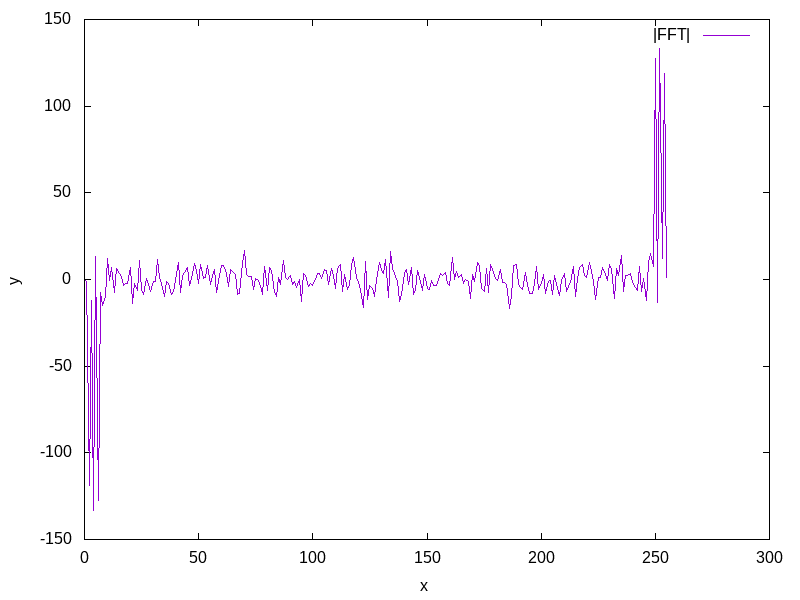
\includegraphics[width=6cm]{k8cz1.jpg}}
\linespread{1.5}
\subfloat[Moduł współczynników transformaty i próg dyskryminacji sygnału na poziomie $max|c_k|/2$ ]{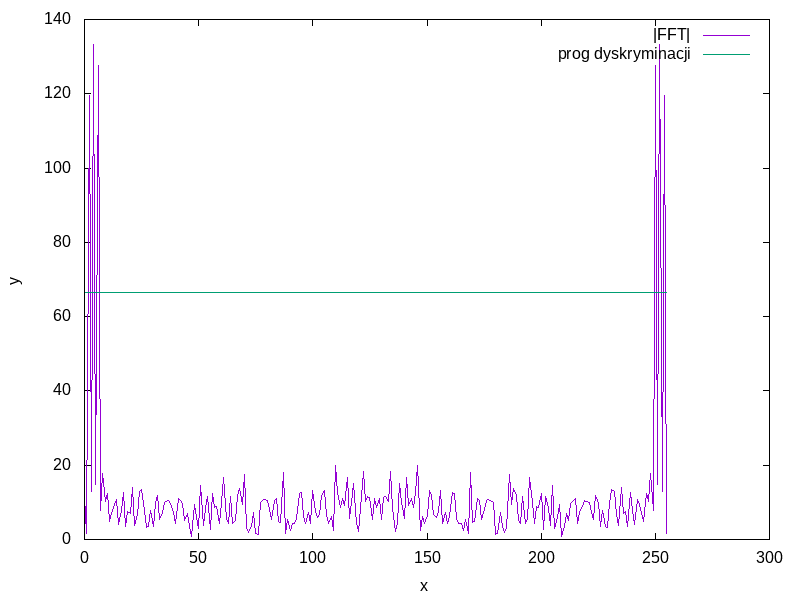
\includegraphics[width=6cm]{k8cz2.jpg}}
\end{figure}
\newline
Wartości, które nie zostały podane dyskryminacji znajdują się na obu krańcach przedziału. 
\newpage
Wyniki sygnału zaburzonego:
\begin{figure}[H]
\centering
\subfloat[$k = 8$, $N_k = 2^8$]{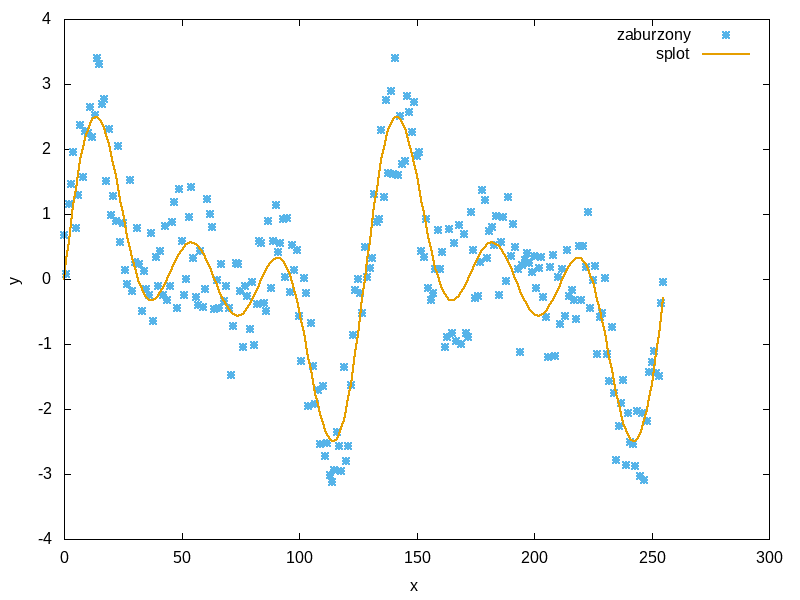
\includegraphics[width=6cm]{k8cz3.jpg}}
\subfloat[$k = 10$, $N_k = 2^{10}$]{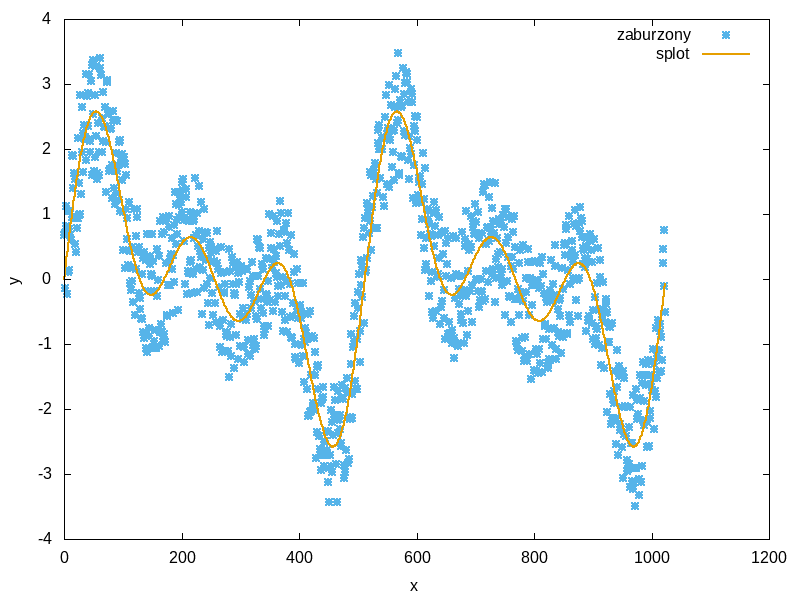
\includegraphics[width=6cm]{k10cz3.jpg}}\\
\subfloat[$k = 12$, $N_k = 2^{12}$]{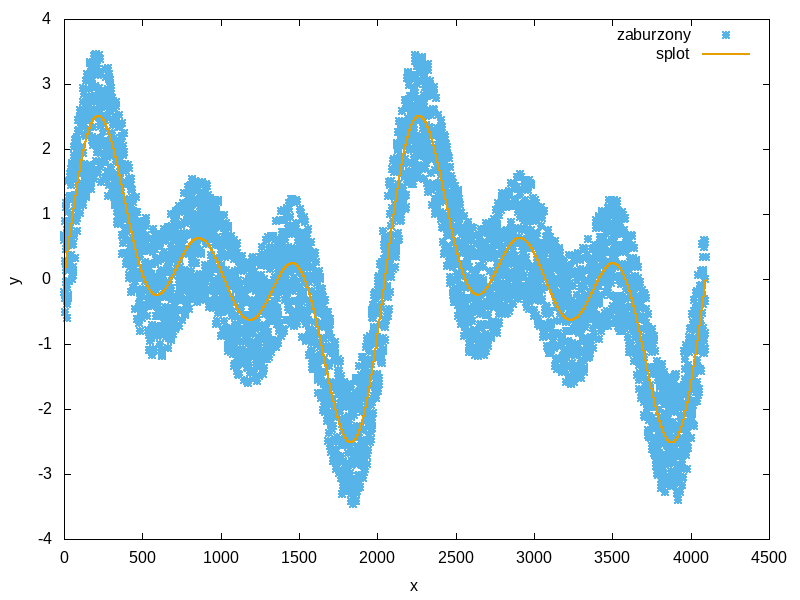
\includegraphics[width=6cm]{k12cz3.jpg}}
\end{figure}

Wyniki sygnału niezaburzonego:

\begin{figure}[H]
\centering
\subfloat[$k = 8$, $N_k = 2^8$]{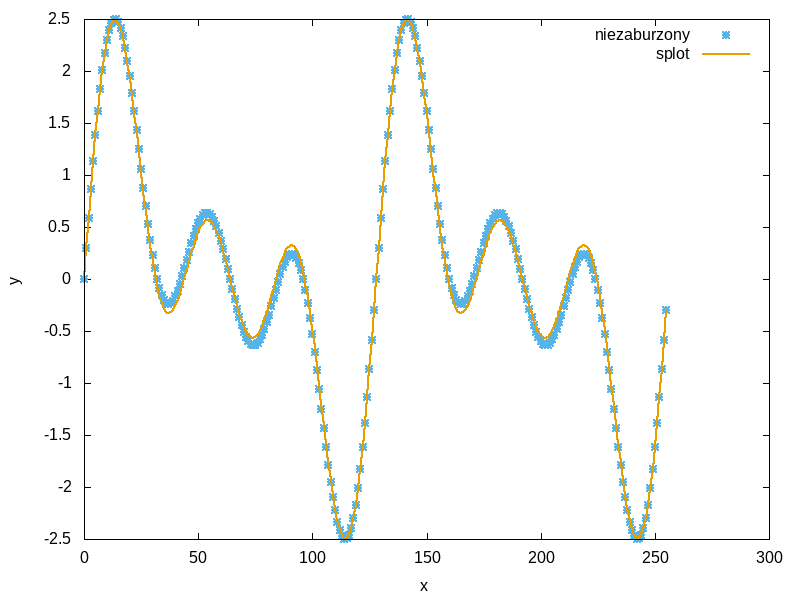
\includegraphics[width=6cm]{k8cz4.jpg}}
\subfloat[$k = 10$, $N_k = 2^{10}$]{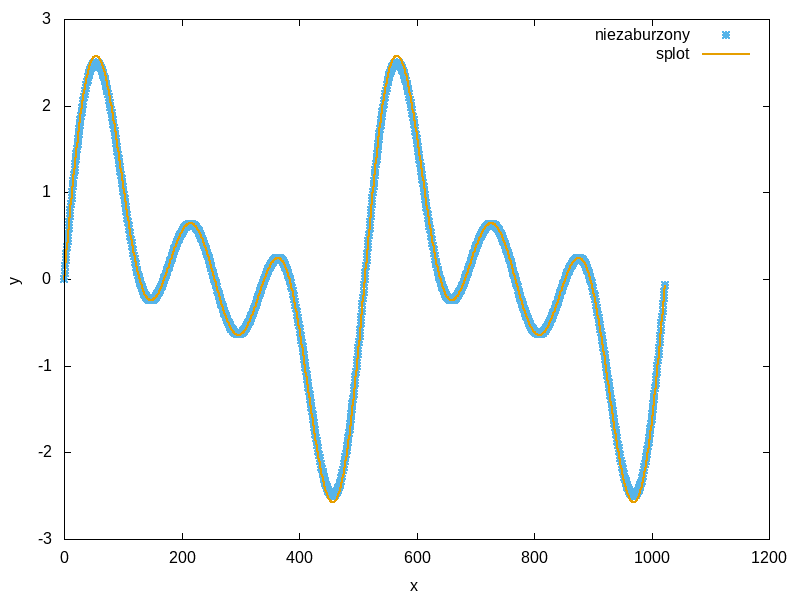
\includegraphics[width=6cm]{k10cz4.jpg}}\\
\subfloat[$k = 12$, $N_k = 2^{12}$]{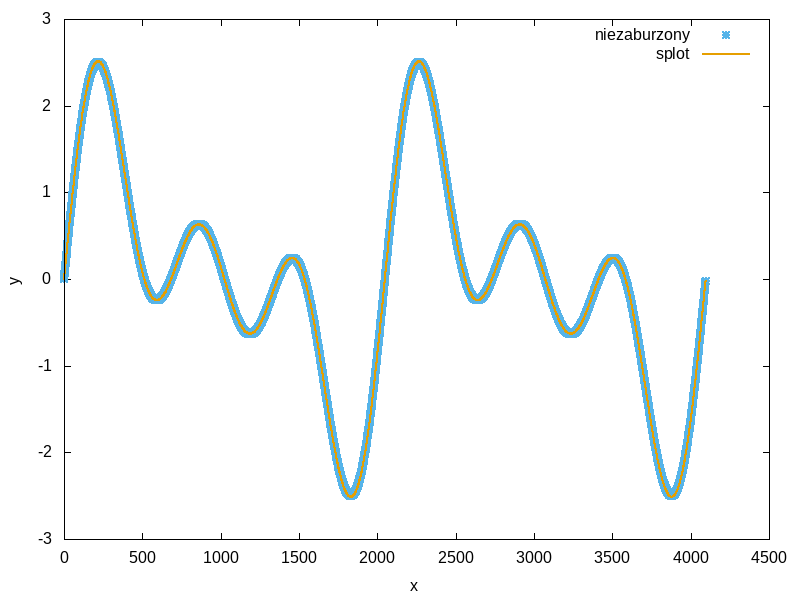
\includegraphics[width=6cm]{k12cz4.jpg}}
\end{figure}
Wykresy po odszumieniu praktycznie pokrywają się z wykresami bez szumów i są bardziej dokładne im większe jest $k$. 

\section{Wnioski}
Jak można zauważyć wybór progu dyskryminacji na połowę modułu maksymalnego współczynnika transformaty daje bardzo zadowalające rezultaty. Dla mniejszych liczb prób w punktach ekstremów lokalnych występowały niedopasowania, a odszumiony wykres nie był idealnie gładki. Dla większej liczby węzłów przybliżenie było bardziej dokładne. Można także podkreślić zaletę jaką jest krótki czas obliczeniowy metody. Szybka Transformacja Fouriera pozwoliła na bardzo dokładne i szybkie przybliżenie funkcji zaszumionej.

\begin{thebibliography}{1}

\bibitem{1}
	Tomasz Chwiej, \emph{Szybka transformacja Fouriera} \\
	\texttt{http://galaxy.agh.edu.pl/$\sim$chwiej/mn/fft\_1819.pdf}	
\bibitem{2}	
	\texttt{https://pl.wikipedia.org/wiki/Dyskretna\_transformata\_Fouriera}

\end{thebibliography}

\end{document}